\section{Summary of Metrics}\label{analysis}

Some basic metrics are based simply on counting the number of interactions or the lines of code of a class. Next, we take a closer look at two studies on metrics on fault-proneness. Build on the basic metrics of the Chapter \ref{related}, divided in class metrics, method metrics and attribute metrics, more detailed aspects are now examined. This provides a summary of many similar metrics compared to related research. First, we look at a study that deals with class cohesion metrics.

\begin{figure}[htbp]
	\centerline{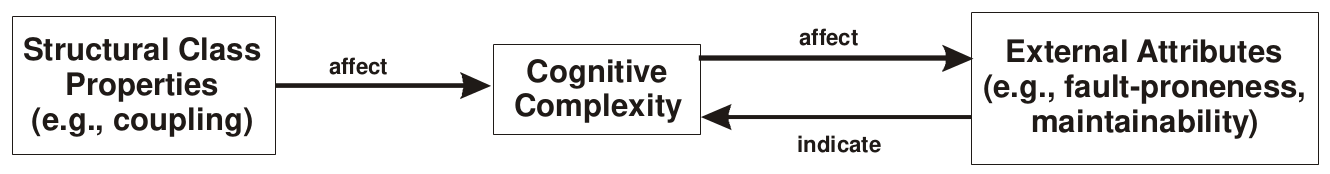
\includegraphics[width=0.5\textwidth]{pictures/faultyclasses1.png}}
	\caption{Theoretical basis for the development of object oriented product metrics \cite{b7radjenovic2013software}.}
	\label{figCoupling}
\end{figure}

\begin{figure}[htbp]
	\centerline{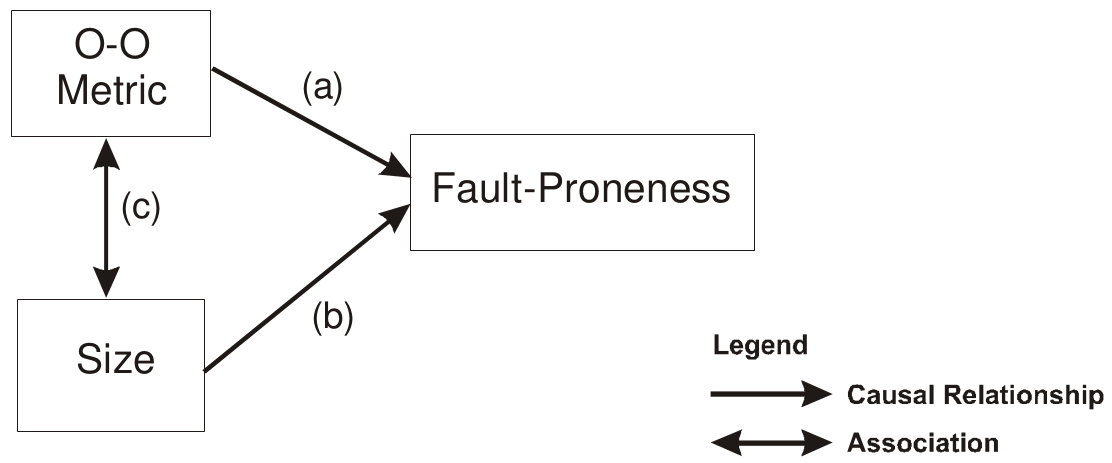
\includegraphics[width=0.45\textwidth]{pictures/faultyclasses2.png}}
	\caption{Path diagram illustrating the confounding effect of class size on the relationship between an object-oriented metric and fault-proneness \cite{b7radjenovic2013software}.}
	\label{figSize}
\end{figure}


\begin{table}
	\caption{Metrics about fault-proneness.}~\label{tab:metrics}
	
	\setlength\tabcolsep{3pt}
	\renewcommand{\arraystretch}{1.4}% for the vertical padding
	\begin{tabularx}{\columnwidth}{ | c | p{5.8cm} || c | }
		\hline
		Abbrevation & Definition & Sources \\ \hline\hline
		LSCC & low-level design class cohesion metric & \cite{b3al2012fault} \\ \hline
		LOC & Lack of Cohesion counts ..  & \cite{b15chidamber1991towards} \\ \hline
		DOI & Depth of Inheritance .. & \cite{b15chidamber1991towards} \\ \hline
		PCCC & path connectivity class cohesion & ... \\ \hline
	\end{tabularx}
\end{table}


\subsection{Method-Method Interaction-Based Cohesion Metrics for Object-Oriented Classes}

Basic units of design in object-oriented programs are classes. Class cohesion refers to the relatedness of class members, i.e., their attributes and methods. Multiple metrics for class cohesion have been proposed in the literature. These object-oriented metrics are based on information available during the high-level or low-level design phases.
In this paper, a formula that accurately measures the degree of interaction between each pair of methods is proposed and used as the basis for introducing a low-level design class cohesion (LSCC) metric \cite{b8al2012precise}. Low-level design (LLD) cohesion metrics use more finely resolved information than that used by High-level design (HLD) cohesion metrics. HLD cohesion metrics identify potential cohesion issues early in the HLD phase. 
In figure \ref{fig1}, rectangles represent methods, circles indicate attributes, and links illustrate the use of attributes by methods of a class. Metrics based on counting the number of links, i.e., the use of attributes by a method, can indicate whether a class is strongly or weakly cohesive. This finely granulated
information is important to help software developers refactoring their code and detecting which methods to possibly remove, i.e., the methods that exhibit even no
links with other methods. When a method-method interaction (MMI) metric
is applied to measure the cohesion for the class shown in figure \ref{fig1}, the
connectivity between each pair of methods is calculated, and it is clearly seen that
method $m_3$ is weakly interconnected to other methods in this class.

\begin{figure}[htbp]
	\centerline{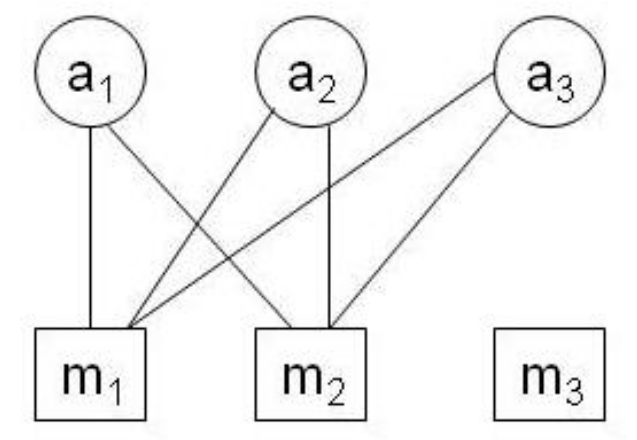
\includegraphics[width=0.2\textwidth]{pictures/am.png}}
	\caption{Sample representative graph for a hypothetical class \cite{b3al2012fault}.}
	\label{fig1}
\end{figure}

As shown in figure \ref{fig2}, there are four other classes with a different method-method interconnection. The class cohesion (CC) of Bonja and Kidanmariam is the ratio of the summation of the similarities between all pairs of methods to the total number of pairs of methods \cite{bonja2006metrics}. The similarity between methods $i$ and $j$ is defined as
\begin{displaymath}
	sim(i,j)=\frac{|I_i \cap I_j|}{|I_i \cup I_j|} ,  
\end{displaymath}
where $I_i$ and $I_j$ are the sets of attributes linked by methods $i$ and $j$, respectivly \cite{b3al2012fault}. In contrast with the class cohesion metric of Pena (SCOM), the calculation is defined as follows
\begin{displaymath}
	sim(i,j)=\frac{|I_i \cap I_j|}{min(|I_i|, |I_j|)} \cdot \frac{|I_i \cup I_j|}{n},  
\end{displaymath}
where $n$ is the number of attributes \cite{fernandez2006sensitive}.
Both CC and SCOM neither consider transitive MMI nor account for inheritance or different method types, and they have not been empirically validated against external quality attributes such as fault occurrences. Of course, there are many other metrics of this kind but the results for the metrics that consider the degree of interaction between each pair of methods are very close to each other \cite{b8al2012precise}.

\begin{figure}[htbp]
	\centerline{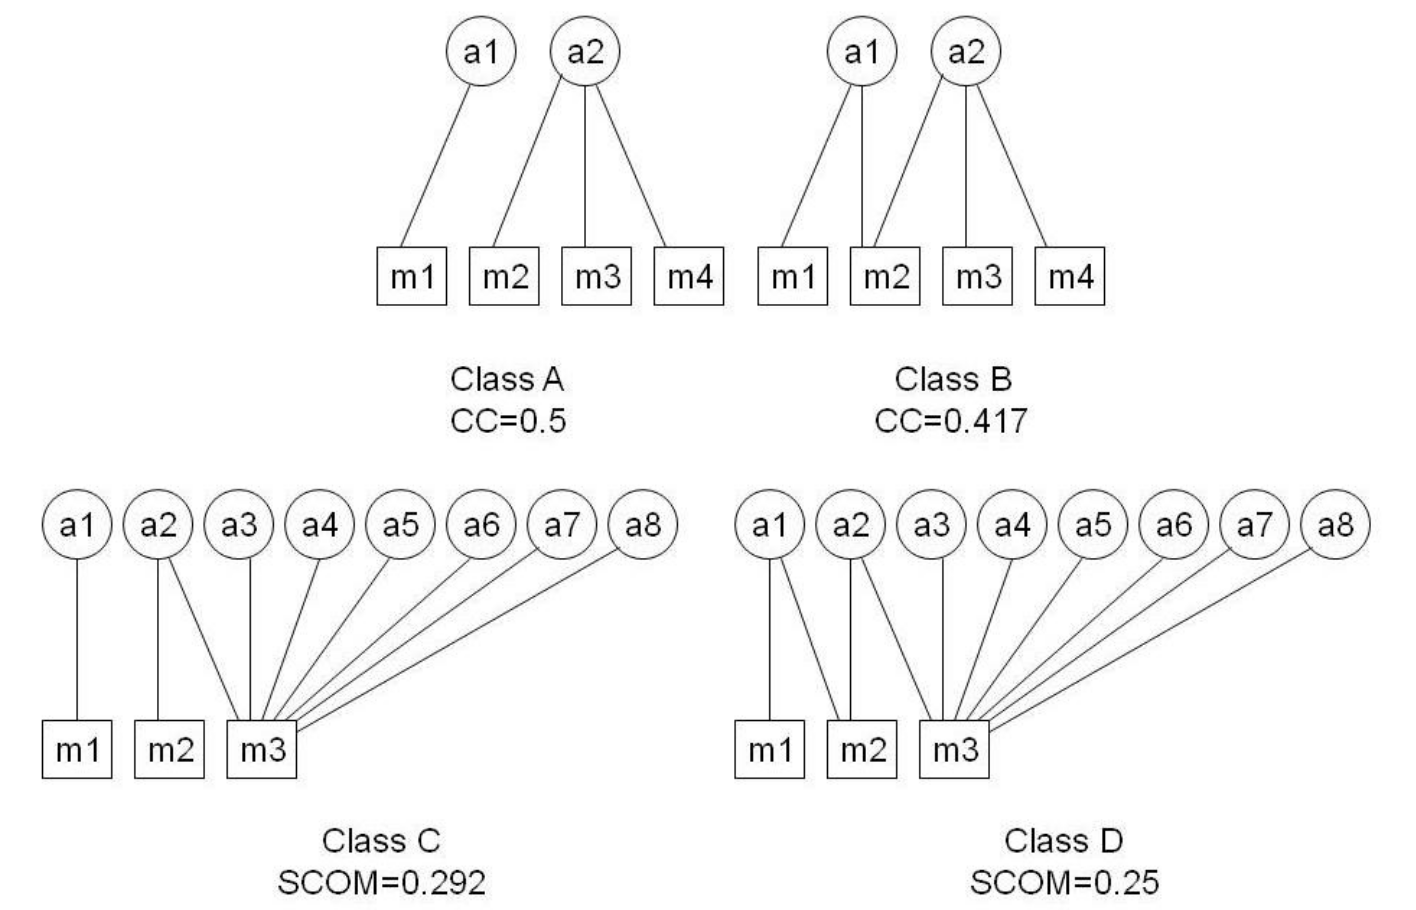
\includegraphics[width=0.4\textwidth]{pictures/am2.png}}
	\caption{Classes with different method-method connectivity patterns \cite{b3al2012fault}.}
	\label{fig2}
\end{figure}

The results suggest that class quality, as measured in terms of fault occurrences, can be more accurately explained by cohesion metrics that account for the degree of interaction between each pair of methods. The fault prediction of interconnection-based object-oriented class cohesion metrics should help the developer to support refactoring during the LLD phase \cite{b8al2012precise}.


\subsection{A Bayesian Network}

The next method to take a closer look at the fault-proneness is a concise representation of a joint probability distribution on a set of statistical variables. Bayesian methods can be used for assessing software fault content and fault proneness. A bayesian network (BN) is encoded as an acyclic graph of nodes and directed edges \cite{b9pai2007empirical}. Assuming that the relationship can be modeled with a general linear model, the structural and numerical specification for the BN is derived. The model can be thought of as a generalization of existing techniques for assessing software quality. The model consists roughly of two parts, first the method produces a probability distribution of the estimated fault content per class in the system and second the conditional probability that a class contains a fault. 
The structure of the model is a BN model whose underlying representation is the generalized linear model. The definition probabilistic network (acyclic graph $G=(V,E)$; A set $S$, of (prior) conditional probability distributions).
Consider a finite set of random variables $X=\{X_1,X_2,....,X_n\}$. It can be defined that a probabilistic network $N=(G,X) over X$ consists of
 \begin{enumerate}
 	\item[-] a directed acyclic graph $G=(V,E)$, $V$ is the set of nodes in the graph and there is a one-one correspondence between $V$ and $X$. $E \subseteq V \times V$ the set of directed edges, representing conditional independence assumptions, i.e., for each $X_i \in X$, $i(X_i,N D_{x_i}| Pa_{x_i})$ and $N D_{x_i} = X \backslash ({X_i} \cup Des_{x_i})$ 
 	\item[-] a set of (prior) conditional probability distributions, that specifies $p(X_i)| p(Pa_{x_i})$ for each $X_i \in X$, where $Pa_{x_i}$ represents the set of immediate parents of $X$.
 \end{enumerate} 

Once a network is specified over a set of random variables, their marginal and joint probabilities can be computed.
Given a BN structure, the joint probability distribution over $X$ is encoded as

\begin{displaymath}
	p(X)= \prod_{i=1}^{n}p(X_i|P_{ax_i})
\end{displaymath}

And given this joint probability, the marginal probability of a random variable $X_i$ is computed as 

\begin{displaymath}
	p(X_i)= \sum_{X_i,j\neq i}^{n}p(X)
\end{displaymath}

The model parameters that are used are listed in the following \cite{b9pai2007empirical}: 

\begin{itemize}
	\item[1.] Weighted methods per class (\textbf{WMC}): The number of methods implemented in a given class.
	\item[2.] Depth of inheritance tree (\textbf{DOI})
	\item[3.] Response for class (\textbf{RFC}): Number of methods implemented within a class plus the number of methods accessible to an object class due to inheritance. (Traditionally, it represents the number of methods that an object of a given class can execute in response to a received message \cite{b9pai2007empirical}.)
	\item[4.] Number of children (\textbf{NOC}): The number of classes that directly inherit from a given class.
	\item[5.] Coupling between object classes (\textbf{CBO}): The number of distinct non-inheritance related classes to which a given class is coupled. (i.e., when a given class uses the methods or attributes of the coupled class \cite{b9pai2007empirical}.)
	\item[6.] Lack of cohesion in methods (\textbf{LCOM}): A measure of the degree to which a class represents single or multiple abstractions. There are varying definitions for LCOM. (i.e., by computing the average percentage of methods in a given class using each attribute of that class, and then subtracting that percentage from 100 percent \cite{b9pai2007empirical}.)
	\item[7.] Source lines of code (\textbf{SLOC}): This is measured as the total lines of source code in the class and serves as a measure of class size.
\end{itemize}

The dependent variables, which serve as surrogate metrics of software quality, are
\begin{itemize}
	\item Fault Content (FC): We define fault content as the number of faults per class. The estimation of ourmodel is a (marginal) conditional probability ofobserving a certain number of faults per class, giventhe metrics for that class.
	\item Fault proneness (FP): The conditional probability thata class contains a fault, given the metrics for that class.
\end{itemize}

\begin{figure}[htbp]
	\centerline{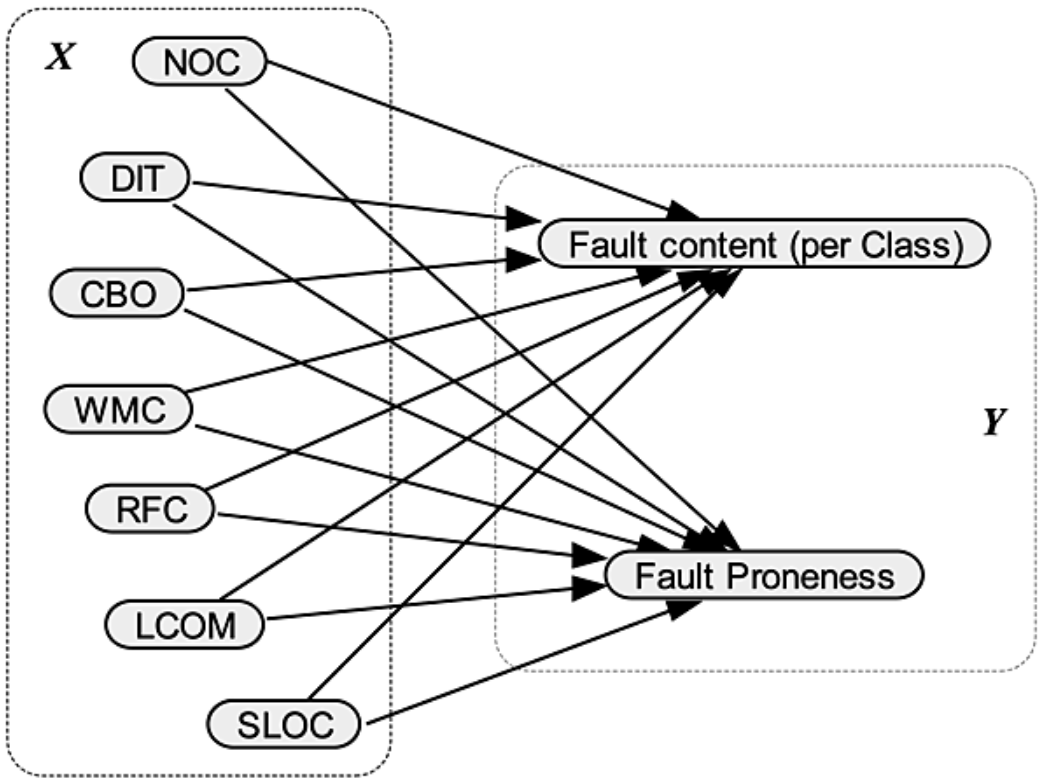
\includegraphics[width=0.4\textwidth]{pictures/bn2.png}}
	\caption{BN model for fault content and fault-proneness analysis.}
	\label{fig2bn}
\end{figure}

The model construction is as follows

\begin{figure}[htbp]
	\centerline{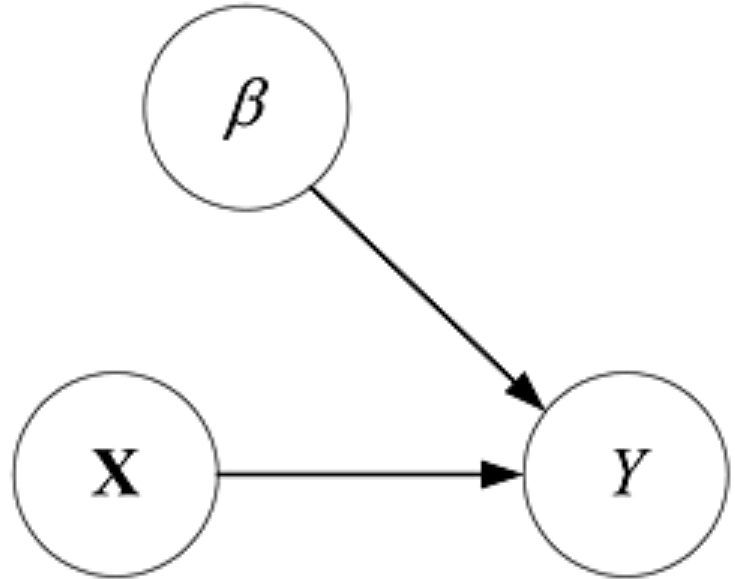
\includegraphics[width=0.2\textwidth]{pictures/bn1.png}}
	\caption{BN representation of a general linear model.}
	\label{fig1bn}
\end{figure}


The results also show that this model producesthese estimations at a statistically significant level.

- RESULTS 

- BN: the results of performing multiple regression, the metrics WMC, CBO, RFC, and SLOC are very significant for assessing both fault content and fault proneness

- this specific set of predictors is very significant for assessing fault content and fault proneness in large software systems

- it was observed that import coupling (that count the number of other classes called by a class) metrics are strongly associated with fault
pron and predict faulty classes with high accuracy

- Associate refactoring to the last sections
